% Template for APA submission with R Markdown

% Stuff changed from PLOS Template
\documentclass[a4paper,man,natbib]{apa6}
\usepackage{apacite}

% amsmath package, useful for mathematical formulas
\usepackage{amsmath}
% amssymb package, useful for mathematical symbols
\usepackage{amssymb}

% hyperref package, useful for hyperlinks
\usepackage{hyperref}

% graphicx package, useful for including eps and pdf graphics
% include graphics with the command \includegraphics
\usepackage{graphicx}

% Sweave(-like)
\usepackage{fancyvrb}
\DefineVerbatimEnvironment{Sinput}{Verbatim}{fontshape=sl}
\DefineVerbatimEnvironment{Soutput}{Verbatim}{}
\DefineVerbatimEnvironment{Scode}{Verbatim}{fontshape=sl}
\newenvironment{Schunk}{}{}
\DefineVerbatimEnvironment{Code}{Verbatim}{}
\DefineVerbatimEnvironment{CodeInput}{Verbatim}{fontshape=sl}
\DefineVerbatimEnvironment{CodeOutput}{Verbatim}{}
\newenvironment{CodeChunk}{}{}

% cite package, to clean up citations in the main text. Do not remove.
\usepackage{cite}

\usepackage{color}

% Use doublespacing - comment out for single spacing
%\usepackage{setspace}
%\doublespacing


% Text layout
\topmargin 0.0cm
\oddsidemargin 0.5cm
\evensidemargin 0.5cm
\textwidth 16cm
\textheight 21cm

% Bold the 'Figure #' in the caption and separate it with a period
% Captions will be left justified
\usepackage[labelfont=bf,labelsep=period,justification=raggedright]{caption}

% Use the APA provided bibtex style
\bibliographystyle{apacite}

% Remove brackets from numbering in List of References
\makeatletter
\renewcommand{\@biblabel}[1]{\quad#1.}
\makeatother


% Leave date blank
\date{}

\pagestyle{myheadings}
%% ** EDIT HERE **


%% ** EDIT HERE **
%% PLEASE INCLUDE ALL MACROS BELOW

%% END MACROS SECTION


% ALL OF THE TITLE PAGE INFORMATION IS SPECIFIED IN THE YAML
\title{\textbf{Using social cues to constrain cross-situational word learning}}
\shorttitle{Social context and cross-situational learning}

\author{Kyle MacDonald, Daniel Yurvosky, and Michael C. Frank}

\affiliation{Department of Psychology, Stanford University}

\authornote{We are grateful to the members of the Language and Cognition Lab for
their feedback on this project. This work was supported by a National
Science Foundation Graduate Research Fellowship to KM and an NIH NRSA
Postdoctoral Fellowship to DY.

Please address correspondence to Kyle MacDonald, Jordan Hall (Building
420), Stanford University, 450 Serra Mall, Stanford, CA 94305. Email:
\href{mailto:kyle.macdonald@stanford.edu}{\nolinkurl{kyle.macdonald@stanford.edu}}.}
\abstract{Both adults and children are capable statistical learners -- able to
track word-object co-occurrences over time to infer word meanings from
ambiguous learning contexts. But word learning is embedded within a
broader social context that includes additional pragmatic cues
(e.g.~gesture, locus of attention) to a speaker's intended meaning. How
do these cues affect statistical word learning? Drawing on
social-pragmatic theories of language acquisition, we hypothesize that
the presence of a referential cue, like gaze, guides how learners
allocate their limited cognitive resources and modulates the underlying
representation used for statistical learning. In three large-scale
experiments with adults, we test how the presence of referential cues
affects cross-situational word learning. Referential cues shift learners
away from multiple hypothesis tracking towards storing only a single
hypothesis (Experiments 1 and 2). In addition, learners are sensitive to
the reliability of a cue and when it is less reliable, they are less
likely to use it and more likely to store multiple hypotheses
(Experiment 3). Together, the data suggest that learners make a rational
tradeoff: In conditions of greater uncertainty, they store a broader
range of information.}
\keywords{statistical learning, pragmatic cues, word learning, language
acquisition}

\begin{document}
\maketitle

``Language is a social act.''

\section{Introduction}\label{introduction}

Learning the meaning of a new word should be hard. Even concrete nouns
are often used in complex contexts with multiple possible referents,
which in turn have many conceptually natural properties that a speaker
could talk about. This inherent ambiguity creates the potential for an
(in principle) unlimited amount of referential uncertainty in the
learning task (Quine,
1960).\footnote{Note that this is a simplified version of Quine's *indeterminacy of reference*: that there are many possible meanings for a word ("Gavigai") that include the referent ("Rabbit") in their extension: "white," "rabbit," "dinner," etc. Quine's broader philosophical point was that there are in fact meanings that are extensionally identical and thus logically indistinguishable. For example, the meanings "rabbit" and "undetached rabbit parts" would always be consistent with the presence of a rabbit, making it impossible to tease apart the speaker's meaning.}
Remarkably, word learning proceeds, with estimates of adult vocabularies
ranging between 50,000 to 100,000 distinct words (P. Bloom, 2002). How
do learners infer and retain such a large variety of word meanings from
data with this kind of uncertainty?

Statistical learning theories offer a solution to this learning problem
by aggregating cross-situational statistics across labeling events to
identify underlying word meanings (Siskind, 1996; Yu \& Smith, 2007).
Recent experimental work shows that both adults and young infants can
use word-object co-occurrence statistics to learn words from
individually ambiguous naming events (L. Smith \& Yu, 2008; Vouloumanos,
2008). For example, L. Smith \& Yu (2008) taught 12-month-olds three
novel words simply by repeating consistent novel word-object pairings
across 10 ambiguous exposure trials. Moreover, computational models
suggest that cross-situational learning can scale up to learn
adult-sized lexicons, even under conditions of considerable referential
uncertainty (K. Smith, Smith, \& Blythe, 2011).

Although all cross-situational learning models agree that the input is
the co-occurrence between words and objects and the output is stable
word-object mappings, they disagree about how closely learners
approximate the input distribution.\footnote{For a detailed discussion
  of these debates, see Smith, Suanda, \& Yu (2014).} Some theories hold
that we accumulate graded, statistical evidence about multiple referents
for each word (McMurray, Horst, \& Samuelson, 2012), while others argue
that we track only a single candidate referent (Trueswell, Medina,
Hafri, \& Gleitman, 2013). Recent experimental and modeling work by
Yurovsky \& Frank (in press) suggests an integrative explanation:
learners allocate a fixed amount of their attention to one hypothesis,
and the rest gets distributed evenly among the remaining alternatives.
As the set of alternatives grows, the amount allocated to each object
approaches zero.

Another ongoing debate in the literature is how to best characterize the
input to cross-situational learning mechanisms. One way researchers have
quantified the ambiguity in the input is to ask adults to guess the
meaning of an intended referent from clips of caregiver-child
interactions (Human Simulation Paradigm: HSP). Using the HSP, Medina,
Snedeker, Trueswell, \& Gleitman (2011) found that adults did not show
evidence of aggregating multiple word--referent correspondences across
trials, concluding that real world learning contexts are too noisy to
support tracking of multiple correspondences over time. In contrast,
Yurovsky, Smith, \& Yu (2013) found a bimodal distribution, with half of
the naming episodes being unambiguous to adults. In addition, Cartmill
et al. (2013) showed that the proportion of unambiguous naming episodes
varies across parents, with some parents' rarely providing highly
informative contexts and others' doing so relatively often.

Thus, representations in cross-situational word learning can appear
distributional or discrete, and the input to statistical learning can
vary along a continuum of ambiguity. These results raise an interesting
question: could learners be sensitive to the ambiguity of the input and
use this information to alter the representations stored in memory? In
the current line of work, we investigate how social information could
affect learners' underlying representations.

Social-pragmatic theories of language learning emphasize the importance
of pragmatic cues for word learning (P. Bloom, 2002; Clark, 2009;
Hollich et al., 2000). Experimental work shows that even children as
young as 16 months are sophisticated intention-readers, preferring to
map novel words to objects that are the target of a speaker's gaze and
not their own (Baldwin, 1993). And in naturalistic observations,
learners tend to retain labels that are accompanied with clear
referential cues that are concurrent with visual access (Yu \& Smith,
2012). Moreover, correlational data show strong links between early
intention-reading skills (e.g., gaze following) and later vocabulary
growth (Brooks \& Meltzoff, 2005, 2008; Carpenter, Nagell, Tomasello,
Butterworth, \& Moore, 1998).

Together, the evidence suggests that referential cues could interact
with the representations underlying statistical word learning. In the
current set of studies, we explore this interaction and ask two
interrelated questions: (1) Does the presence of a valid referential cue
modulate ambiguity in the learning context? (2) Do learners' flexibly
alter their representations of alternative referents in response to
different levels of contextual ambiguity?

To answer these questions, we use a modified version of Yurovsky \&
Frank (in press)`s paradigm to test the hypothesis that the presence of
a social cue, a speaker's gaze, will alter learners' allocation of
attention and reduce the number of word-object links that are stored in
memory. In Experiment 1, we manipulate the presence of a referential cue
at different levels of attention and memory demands. At all levels of
difficulty, learners tracked a strong single hypothesis, but learners
were less likely to track multiple word-object links when referential
cues were present. In Experiment 2, we replicate the findings from
Experiment 1 with a more ecologically valid stimulus set. In Experiment
3, we show that reducing the reliability of the referential cue
increases learners multiple hypothesis tracking, providing evidence that
learners were sensitive to a graded manipulation of the quality of the
learning context. In sum, the data suggest that learners adaptively
allocate attention and store representations with different levels of
fidelity depending on the amount of referential uncertainty present
during learning.

\section{Experiment 1}\label{experiment-1}

We set out to test the effects of referential cues on cross-situational
learning at different levels of attention and memory demands.
Participants saw a series of ambiguous exposure trials that consisted of
a set of novel objects (either 2, 4, 6, or 8) and an image of a
schematic, female interlocutor. On each trial they heard one novel word
that was either paired with an gaze cue or not, and were asked to make
guesses about which object went with each word. In subsequent test
trials, participants heard the novel word again after different numbers
of intervening trials (0, 1, 3, and 7), this time paired with a new set
of novel objects. Importantly, test trials were contingent upon
participants' selection during exposure such that one of the objects in
the set was either the participant's initial guess (Same trials) or one
of the objects that was \emph{not} the initial guess (Switch trials).
While both single and multiple referent trackers could succeed on Same
trials, only participants who encoded multiple word-object links during
their first encounter could succeed on Switch trials. This provides a
direct measure of whether learners track multiple alternatives and if
these representations are influenced by the presence of referential
cues.

\subsection{Method}\label{method}

\subsubsection{Participants}\label{participants}

This experiment was posted to Amazon Mechanical Turk as a set of Human
Intelligence Tasks (HITs) to be completed only by participants with US
IP addresses and an approval rate above 95\%. Each HIT paid 30 cents.
Approximately 50-130 HITs were posted for each of the 32 conditions (4
referents X 4 intervals X 2 gaze conditions) for total of approximately
2400 paid HITs. If a participant completed the experiment more than
once, he or she was paid each time but only data from the first HITs
completion was included in the final data set. In addition, data was
excluded from the final sample if participants did not give correct
answers for familiar trials (5 HITs excluded).

\begin{CodeChunk}
\begin{figure}
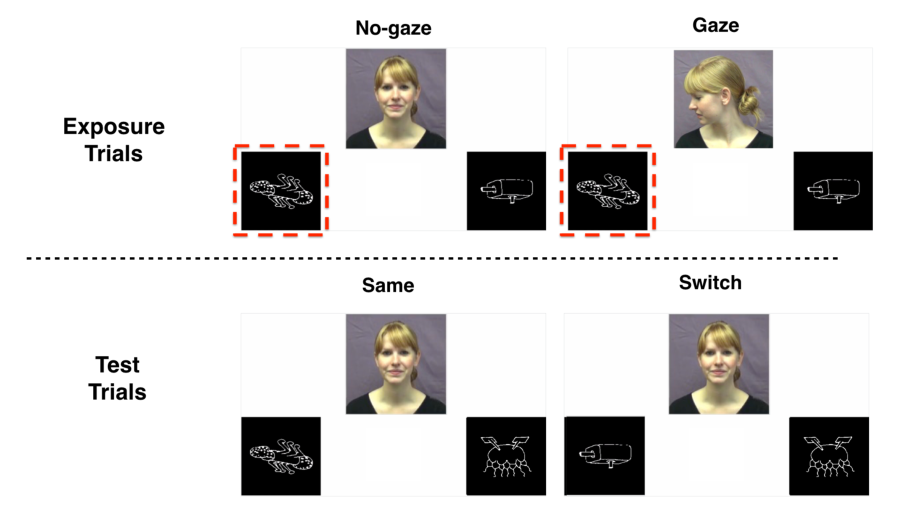
\includegraphics{figs/stimuli-1} \caption[Examples of exposure and test trials from Experiment 1 (schematic gaze cue) and Experiments 2/3 (live action gaze cue)]{Examples of exposure and test trials from Experiment 1 (schematic gaze cue) and Experiments 2/3 (live action gaze cue). Participants saw exposure trials with or without a gaze cue depending on condition assignment. All participants saw both types of test trials: same and switch. On same trials the object that participants chose during exposure appeared with a new novel object. On switch trials the object that participants did not choose appeared with a new novel object.}\label{fig:stimuli}
\end{figure}
\end{CodeChunk}

\begin{CodeChunk}
\begin{figure}
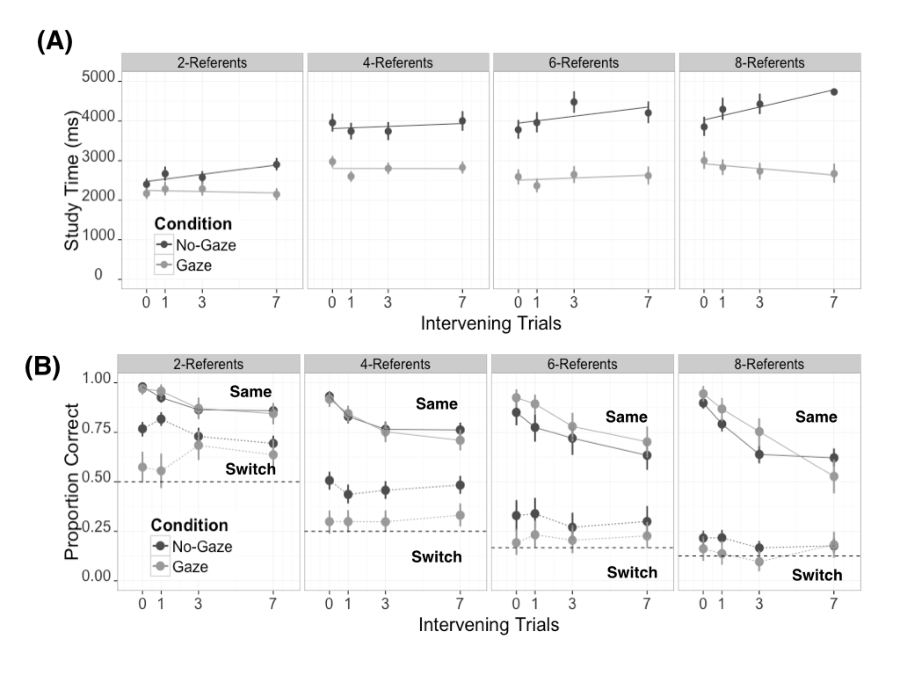
\includegraphics{figs/expt1-plot-1} \caption[Experiment 1 results]{Experiment 1 results. Panel A shows study time on exposure trials across all experimental conditions: gaze and no-gaze, number of referents (2, 4, 6, and 8), and number of intervening trials (0, 1, 3, and 7). Panel B shows accuracy on test trials for both trial types (Same and Switch) across all conditions. Error bars indicate 95\% confidence intervals computed by non-parametric bootstrap.}\label{fig:expt1-plot}
\end{figure}
\end{CodeChunk}

\subsubsection{Stimuli}\label{stimuli}

Figure 1 shows stimuli used in Experiment 1. These stimuli consisted of
black and white pictures of familiar and novel objects drawn from the
set of 140 first used in Kanwisher, Woods, Iacoboni, \& Mazziotta
(1997), a schematic drawing of a human interlocutor, and audio
recordings of familiar and novel words. Familiar words consisted of the
labels for the familiar objects as produced by AT\&T Natural Voices
\texttrademark (voice: Crystal). Novel words were 1-3 syllable
pseudowords obeying the rules of English phonotactics produced using the
same speech synthesizer. A schematic drawing of a human speaker was
chosen for ease of manipulating the direction of gaze, the referential
cue of interest in this study.

\subsubsection{Design and Procedure}\label{design-and-procedure}

Participants were exposed to a series of 16 trials (8 exposure, and 8
test) in which they heard a speaker say one novel word, saw a set of
novel objects, and were asked to guess which object went with the word.
After a written explanation of the task, participants completed four
practice trials that consisted of familiar words and objects. These
trials also served to screen for participants who did not have their
audio enabled or who were not attending to the task.

After the practice trials, participants were informed that they would
now hear novel words, and see novel objects, and that they should
continue selecting the correct referent for each word. Participants
heard eight novel words twice, one exposure and one test trial for each
word. Four of the test trials were \emph{Same} trials in which the
object that participants selected on the exposure trial appeared again
amongst a set of new objects. The other four were \emph{Switch} trials
in which one of the objects in the set was selected randomly from the
objects that the participant did not select on the previous exposure
trial. All other objects were completely novel on each trial.

Participants were randomly assigned to see either 2, 4, 6, or 8
referents on each trial and to have either 0, 1, 3, or 7 trials in
between exposure and test. Participants were also assigned to either the
Gaze or No-gaze condition. In the Gaze condition, gaze was directed
towards one of the objects on exposure trials; in the No-gaze condition,
gaze was always directed straight ahead. On test trials, gaze was never
informative. To indicate that participants' selections had been
registered, a red dashed box appeared around the object they selected
for one second after their click was received. This box appeared around
the selected object whether or not it was the ``correct'' referent.

\subsection{Results and Discussion}\label{results-and-discussion}

\subsubsection{Exposure trials}\label{exposure-trials}

To ensure that our referential cue manipulation was effective we
compared participant's performance on Exposure trials in the gaze
condition against the distribution expected if participants were
selecting randomly (defined by a Binomial guessing model with four
trials and a probability of success of \(\frac{1}{Num Referents}\)). In
all conditions, participants' responses differed from those expected by
chance, exact binomial p(two-tailed) \textless{} .001, suggesting that
gaze effectively directed participants' attention to the target
referent.

We also analyzed participants' response times on exposure trials, which
were self-paced and thus a proxy for attention allocated to the
referents on the screen. Panel A of Figure 2 shows participants'
response times across all conditions. We fit a linear mixed effects
model\footnote{All models were fit using the lme4 package in R (Bates,
  Maechler, Bolker, \& Walker, 2013).} as follows:
\(RT \sim Gaze \times Log(Interval) \times Log(Referents) + (Trial \, type \mid subject)\).
We found a significant main effect of referents (\(\beta = 806.95\), p
\textless{} .001) with slower responses as the number of referents
increased. We also found a significant two-way interaction between gaze
condition and number of referents (\(\beta = -517.43\), p \textless{}
.001) such that responses were faster in the gaze condition, especially
as the number of referents increased. This analysis provides evidence
that the presence of a referential cue focused participants' attention
away from alternative word-object links.

\subsubsection{Test trials}\label{test-trials}

To analyze performance on Test trials, we compared the distribution of
correct responses made by each participant to the distribution expected
if participants were selecting randomly. Figure 2 shows participants'
accuracies in identifying the referent of each word in all conditions
for both kinds of trials (Same and Switch) and in each referential cue
condition (Gaze and No-gaze). We replicate the finding from Yurovsky \&
Frank (in press): at all Referent and Interval levels, both for Same and
for Switch trials, participants' responses differed from those expected
by chance (smallest \(\chi^2\) 2(4) = 12.07, p \textless{} .01).
Participants' success on Switch trials provides direct evidence that
learners encoded more than a single hypothesis in ambiguous word
learning situations, even under high attentional and memory demands.

To quantify the effect of each factor on the likelihood of a correct
response, we fit a mixed-effects logistic regression model to the full
dataset as follows:
\(Accuracy \sim Trial type \times Gaze \times Log(Interval) \times Log(Referents) + (Trial \, type \mid subject)\).
We found significant main effects of number of referents
(\(\beta = -0.66\), p \textless{} .001) and interval (\(\beta = -0.49\),
p \textless{} .001), such that as each of these factors increased,
accuracy on test trials decreased. We also found significant main
effects of trial type (\(\beta = -1.3\), p \textless{} .001), with worse
performance on switch trials.

Next we examined the interactions between each factor. There were
significant two-way interactions between trial type and interval
(\(\beta = 0.32\), p \textless{} .001) and trial type and number of
referents (\(\beta = -0.69\), p \textless{} .001) such that the interval
between exposure and test affected same trials more than switch trials,
and the number of referents affected switch trials more than same
trials. The two-way interaction between trial type and gaze condition
was not significant in this model, but trended in the correct direction
(\(\beta = -0.52\), p = 0.13).

The interaction between trial type and gaze condition is the critical
test of our hypothesis because it shows that the presence of a
referential cue reduced learners multiple hypothesis tracking, resulting
in lower accuracy scores on switch trials. But we would only expect to
see this effect if participants were actually following the gaze cue on
exposure trials. Thus, we fit a mixed-effects logistic regression to a
filtered dataset, removing those participants who were not reliably
selecting the referent that was the target of gaze on exposure trials.
This filter removed 90 participants who selected the gaze target at
below chance levels on exposure trials. The analysis of the filtered
dataset showed a reliable interaction between trial type and gaze
condition (\(\beta = -0.8\), p \textless{} .05), with worse performance
on switch trials in the gaze condition.

Taken together, the response time and accuracy analyses provide evidence
that learners use of a referential cue modulated their attention during
learning, thus making them less likely to track multiple word-object
links. Interestingly, we did not see strong evidence that reduced
tracking of alternatives resulted in improved performance on same
trials. This finding suggests that the limitations on same trials may be
different than those regulating the distribution of attention on switch
trials, since the presence of a referential cue selectively reduced
learners tracking of alternatives but apparently did not lead learners
to form a stronger memory of their single candidate hypothesis.

It is important to point out that participants' tendency to \emph{use}
the referential cue modulated the effect of gaze on attention and memory
in this experiment. It is interesting that a subset of the particpants
did not reliably use gaze to make their selections on exposure trials.
Perhaps, the effect of gaze was reduced in our experiment because the
referential cue that we used -- a static schematic drawing of a speaker
-- was relatively weak compared to the cues present in real world
learning environments. Hence, we do not yet know whether learners'
cross-situational learning change in the presence of a stronger and more
ecologically valid referential cue. Our next experiment tests this
hypothesis.

\section{Experiment 2}\label{experiment-2}

In Experiment 2, we attempt to replicate the findings from Experiment 1
using a more ecologically valid stimulus set. To move closer to a real
word referential cue, we replaced the static, schematic gaze cue with a
live actress and introduced a within-subjects design where each
participant saw both gaze and no-gaze exposure trials. We selected a
subset of conditions from Experiment 1, testing only the 4-referent
display with 0 and 3 intervening trials as between-subjects
manipulations. Our goals were to replicate the reduction in learners'
multiple hypothesis tracking in the presence of referential cues, and to
test whether increasing the ecological validity of the cue would result
in a boost to the strength of learners' recall of their single candidate
hypothesis.

\subsection{Method}\label{method-1}

\subsubsection{Participants}\label{participants-1}

Participant recruitment and inclusionary/exclusionary criteria were
identical to those of Experiment 1 (excluded 36 HITs). 100 HITs were
posted for each condition (1 referent X 2 intervals X 2 gaze conditions)
for total of 400 paid HITs.

\subsubsection{Stimuli}\label{stimuli-1}

Audio and picture stimuli were identical to Experiment 1. The
referential cue in the gaze condition was a film of a live actress (see
Figure 1). On each exposure trial, the actress looked out at the
participant with a neutral expression, smiled, and then turned to look
at one of the four images on the screen. She maintained her gaze for 3
seconds before returning to the center. On test trials, she looked
straight ahead for the duration of the trial.

\subsection{Design and Procedure}\label{design-and-procedure-1}

Procedures were identical to those of Experiment 1. The major design
change was a within-subjects manipulation of the gaze cue. That is,
participants saw exposure trials with and without gaze. The experiment
consisted of 32 trials broken down into 2 blocks of 16 trials. Each
block consisted of 8 exposure trials and 8 test trials (4 same test
trials and 4 switch test trials), and contained only gaze or no-gaze
exposure trials. The order of block was counterbalanced across
participants.

\subsection{Results and Discussion}\label{results-and-discussion-1}

We followed the same analysis plan as in Experiment 1. First, we analyze
performance on exposure trials to ensure that participants were using
the referential cue and to test if the cue changed response times. Then
we analyze performance on test trials to measure the effect of the
presence of referential cues on the number of word-object links learners
stored in memory.

\subsubsection{Exposure trials}\label{exposure-trials-1}

Similar to Experiment 1, participants' responses on exposure trials
differed from those expected by chance, exact binomial p(two-tailed)
\textless{} .001, suggesting that gaze was effective in directing
attention to the target referent. Participants in Experiment 2 were
numerically more consistent in their use of gaze with the live action
stimuli compared to the schematic stimuli used in Experiment 1 (M1 =
.76, M2 = .81). Panel A of figure 3 shows participants' response times.
We replicate the effect of effect gaze, with faster response times in
gaze condition. We fit a linear mixed effects model to response times
with the same specification as Experiment 1, finding main effects for
gaze condition (\(\beta = -1112.83\), p \textless{} .001) and interval
(\(\beta = -498.96\), p \textless{} .001) with faster responses in the
gaze condition and in the the longer interval condition. The two-way
interaction between gaze condition and interval was not significant,
showing that gaze had the same effect on participants' response times at
both intervals.

\begin{CodeChunk}
\begin{figure}
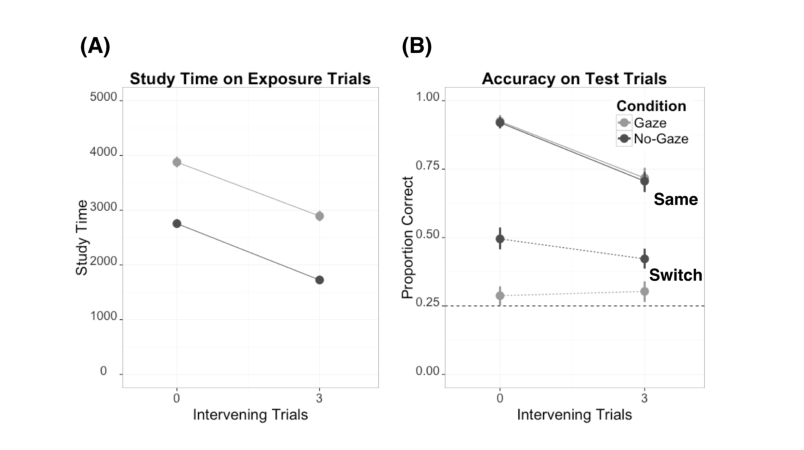
\includegraphics{figs/expt2-plot-1} \caption[Experiment 2 results]{Experiment 2 results. Panel A shows study times for exposure trials. Panel B shows accuracy on test trials. Each datapoint represents 182 participants. Error bars indicate 95\% confidence intervals computed by non-parametric bootstrap.}\label{fig:expt2-plot}
\end{figure}
\end{CodeChunk}

\subsubsection{Test trials}\label{test-trials-1}

Panel B of figure 3 shows performance on test trials in Experiment 2. We
replicate the critical finding from Experiment 1: after seeing gaze
exposure exposure trials participants stored fewer word-object links and
performed worse on switch trials. We fit a mixed-effects logistic
regression model and found significant main effects of interval
(\(\beta = -0.59\), p \textless{} .001) and trial type
(\(\beta = -2.74\), p \textless{} .001). Participants were less accurate
as the interval between exposure and test increased and on the switch
trials overall.

In addition, the model showed a significant two-way interaction between
trial type and interval (\(\beta = 0.51\), p \textless{} .001), with
worse performance on switch trials at the higher interval, and a
marginal two-way interaction betwen gaze condition and interval
(\(\beta = 0.09\), p = 0.07) such that the number of intervening trials
had a smaller effect on participants' performance in the gaze condition.
Importantly, the model showed a reliable interaction between gaze
condition and trial type (\(\beta = -0.73\), p \textless{} .001) with
switch trials being more difficult after gaze exposure trials.
\footnote{We fit models to both the unfiltered and filtered datasets and found no difference between the two analyses, suggesting that increasing the ecological validity of the referential cue and switching to a within-subjects design reduced noise in our measurements.}
Similar to Experiment 1, we did not find evidence of a boost to
performance on same trials in the gaze condition.

Taken together, the data from Experiment 1 and 2 suggest that the
presence of a referential cue reliably focuses learners' attention away
from alternative word-object links and shifts them towards single
hypothesis tracking strategy. Changing to a live action stimulus set led
to slightly higher rates of selecting the target of gaze on exposure
trials, but did not result in a boost to performance on Same trials,
providing additional evidence that the fidelity of participants' single
hypothesis was unaffected in our paradigm by the presence of a
referential cue.

Thus far we have shown that people store different amounts of
information in response to a categorical manipulation of referential
uncertainty: in both Experiments 1 and 2, the learning contexts were
either entirely ambiguous or entirely certain. However, not all real
world learning contexts fall at the extremes of this continuum. Could
learners be sensitive to more subtle changes in the quality of learning
contexts? In our next experiment, we test whether learners store
different amounts of information in response to a \emph{graded}
manipulation of referential uncertainty. This provides an important test
for our account that learners can move along a continuum of
cross-situational word learning strategies, from single to multiple
hypothesis tracking.

\section{Experiment 3}\label{experiment-3}

In Experiment 3, we explore the effects of a parametric manipulation of
referential cues on cross-situational word learning. To accomplish this,
we varied the reliability of the gaze cue. This design was inspired by
experimental work showing that learners are sensitive to the prior
reliability of speakers and use this information when deciding whom to
ask for new information (Koenig, Cl{é}ment, \& Harris, 2004). By
parametrically manipulating reliability, we hoped to test a clear
prediction of our account: that learners will allocate attention and
memory rationally in response to graded changes in the referential
uncertainty present during learning.

\subsection{Method}\label{method-2}

\subsubsection{Participants}\label{participants-2}

Participant recruitment, and inclusionary/exclusionary criteria were
identical to those of Experiment 1 and 2 (excluded 4 HITs). 50 HITs were
posted for each reliability level (0\%, 25\%, 50\%, 75\%, and 100\%) for
total of 250 paid HITs.

\subsubsection{Design and Procedure}\label{design-and-procedure-2}

Procedures were identical to those of Experiment 1 and 2. We modified
our cross-situational learning paradigm to include a block of 16
familiarization trials (8 exposure and 8 test), which established the
reliability of the referential cue. To establish reliability, we varied
the proportion of same/switch trials that occurred during this
familiarization block. Switch trials provide evidence that gaze is not a
reliable predictor of the object that will appear at test. Participants
either saw 0, 2, 4, 6, or 8 switch trials. After the familiarization
block, participants completed a block of 16 trials (8 exposure and 8
test). Importantly, since we were no longer testing the effect of
presence or absence of referential cues, all exposure trials in
Experiment 3 included gaze, but this cue was more or less reliable
depending on which familiarization block participants saw.

\subsection{Results and Discussion}\label{results-and-discussion-2}

\subsubsection{Exposure trials}\label{exposure-trials-2}

First, we analyzed exposure trials across both familiarization and test
blocks. Similar to Experiments 1 and 2, as a group participants reliably
chose the referent that was the target of gaze at rates greater than
those that would be predicted by a guessing model p(two-tailed)
\textless{} .001. Next we analyzed exposure trials in the
post-familiarization block to see if participants were sensitive to our
reliability manipulation. We fit a mixed effects linear regression model
and found a significant effect of reliability level (\(\beta = 1.39\), p
\textless{} .001) such that as the reliability of the gaze cue during
familiarization increased, participants were more likely to select the
target of gaze on exposure trials in the post-familiarization block.
Thus, learners were sensitive to the reliability of the gaze cue.

\begin{CodeChunk}
\begin{figure}
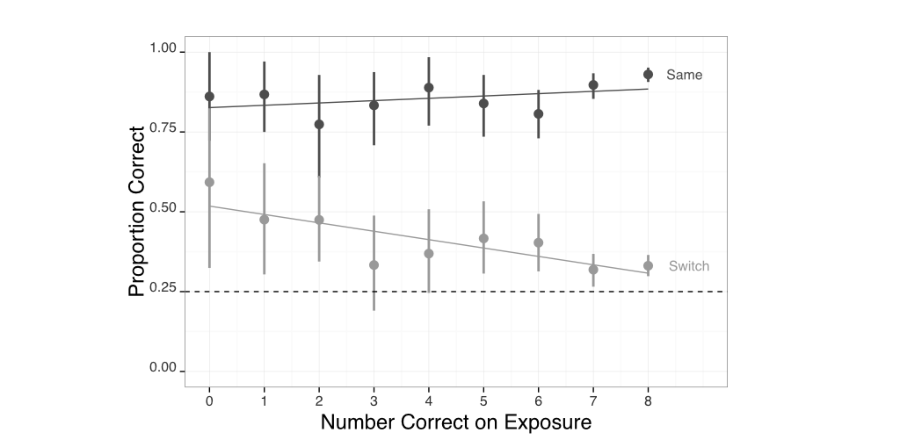
\includegraphics{figs/expt3-plot-1} \caption[Accuracy on test trials in Experiment 3 for both trial types (Same and Switch) as a function of participants' use of gaze on exposure trials]{Accuracy on test trials in Experiment 3 for both trial types (Same and Switch) as a function of participants' use of gaze on exposure trials. Each datapoint represents approximately 50 participants. Error bars indicate 95\% confidence intervals computed by non-parametric bootstrap.}\label{fig:expt3-plot}
\end{figure}
\end{CodeChunk}

\subsubsection{Test trials}\label{test-trials-2}

Figure 4 shows participants accuracy on test trials within the test
block. To quantify the effect of reliability on accuracy, we fit a
mixed-effects logistic regression model and found a significant main
effect of trial type (\(\beta = -2.25\), p \textless{} .001), with
participants responding less accurately on switch trials. In this
analysis, we found a trend towards a significant interaction between
reliability and trial type (\(\beta = -0.72\), p = 0.11).

Similar to Experiment 1, we would only expect to see an interaction
between reliability and trial type if learners used the gaze cue during
exposure trials. Thus, we conducted a follow-up analysis where we
modeled accuracy on test trials as a function of how often participants
chose the target of gaze on exposure trials. We fit a mixed effects
logistic regression model with the same specifications, but substituting
accuracy on exposure trials for reliability condition as a predictor.
With this analysis we found a robust two-way interaction between
performance on exposure trials and trial type (\(\beta = -0.32\), p
\textless{} .001) such that participants who were more likely to use the
gaze cue performed worse on switch trials, but not same
trials.\footnote{Initially, this analysis was post-hoc. So we ran a follow-up study, with all results reported here from a planned analysis of that follow-up experiment.}
These analyses show that as a referential cue becomes more reliable,
participants were more likely to use it, and that learners who used the
referential cue were less likely to store multiple word-object links.

The findings from Experiment 3 support and extend the results of
Experiments 1 and 2 in several ways. First, participants' performance on
same trials was again relatively unaffected by changes in peformance on
switch trials. This provides converging evidence that the limitations on
same trials may be different than those regulating the distribution of
attention on switch trials. Second, it was learners' \emph{use} of a
referential cue that predicted a reduction in memory for alternative
word-object links. It is important to note that although we found a
significant effect of reliability on participants' use of the gaze cue,
participants still tendency to use the cue remained high, even in the
0\% reliability condition (M = 0.81). It is reasonable that participants
would continue to use the gaze cue in our experiment because it was the
only cue available and participants did not have reason to think the
speaker would be deceptive.

The critical contribution of Experiment 3 is the finding that learners
respond to a \emph{graded} manipulation of referential uncertainty, with
the amount of information stored from the intital exposure tracking with
both the reliability of the cue and participants' use of the cue. This
provides support for a critical prediction of our account: that learners
store a strong single candidate word meaning and a set of alternatives
with different levels of fidelity depending the amount of referential
uncertainty present during the initial exposure to a word.

\section{General Discussion}\label{general-discussion}

An ideal statistical learner with unlimited attention and memory could
track all possible word-object co-occurrences, making cross-situational
word learning a simple problem of getting enough data points. But human
learners are constrained by limited cognitive resources, making it
important to decide which statistics to store from an individual
learning moment. Models of cross-situational learning disagree about how
much information is actually stored in memory, with recent work
suggesting that learners maintain both a strong candidate hypothesis and
a set of weaker alternative word-object links (Yurovsky \& Frank, in
press).

Our results suggest that the representations underlying
cross-situational learning are quite flexible. In the absence of a
referential cue to word meaning, learners were more likely to store
alternative word-object links. In contrast, when gaze was present, they
stored less information, showing behavior consistent with tracking a
single hypothesis (Experiments 1 and 2). Learners were also sensitive to
a parametric manipulation of the referential cue, showing a graded
increase in the tendency to use the cue as reliability increased, which
in turn resulted in a graded decrease in memory for alternative
word-object links (Experiment 3). Interestingly, across all three
experiments, reduced memory for alternative hypotheses did not result in
a boost in memory for learners' candidate hypothesis. This pattern of
data suggests that the presence of a referential cue selectively
affected one component of the underlying representation: the number of
alternative word-object links, and not learners candidate hypothesis.

Why did we not see an increase in the strength of learners' candidate
hypothesis? One possibility is that participants did not shift their
cognitive resources from the set of alternatives to their single
hypothesis, but instead rationally conserved their resources for future
use. Griffiths, Lieder, \& Goodman (2015) formalize this behavior by
pushing the rationality of computational-level models down to the
psychological process level. In their framework, cognitive systems are
thought to be adaptive in that they optimize the use of their limited
resources, taking the cost of computation (e.g., opportunity cost of
time or mental opportunity) into account. For example, Vul, Goodman,
Griffiths, \& Tenenbaum (2014) showed that as time pressure increased in
a decision-making task, participants were more likely to show behavior
consistent with a less cognitively challenging strategy of matching,
rather than with the globally optimal strategy. Here, we show evidence
that learners adapt their allocation of cognitive resources to the level
of referential uncertainty in the learning context, spending less time
studying alternative word-object links and reducing the number of links
stored in memory when uncertainty is low.

Our results also fit well with recent experimental work that
investigates how attention and memory can constrain infants' statistical
word learning. For example, Smith \& Yu (2013) used a modified
cross-situational learning task to show that only infants who disengaged
from a novel object to look at both potential referents were able to
learn the correct word--object mappings. Moreover, Vlach \& Johnson
(2013) showed that 16-month-olds were only able to learn from adjacent
cross-situational co-occurrence statistics, and unable to learn from
co-occurrences that were separated in time. Both of these findings make
the important point that only the data that comes into contact with the
learning system can be used for cross-situational word learning, and
this data is directly influenced by the attention and memory constraints
of the learner. Our findings suggest that referential cues could play an
important role in focusing learners' limited attention to the relevant
statistics in the input.

How should we characterize the effect of social information on attention
and memory in our task? One possibility is that the referential cue acts
as a filter, only allowing likely referents to contact statistical
learning mechansims (Yu \& Ballard, 2007). This `filtering account'
separates the effect of social cues from the underlying computation that
aggregates cross-situational information. Another possibility is that
referential cues provide evidence about a speaker's communicative intent
(Frank, Goodman, \& Tenenbaum, 2009). In this model, the learner is
reasoning about the speaker and word meanings simultaneously, which
places inferences based on social information as part of the underlying
computation. A third possibility is that participants thought of the
referential cue as pedagogical. In this scenario, learners assume that
the speaker will choose an action that is most likely to increase the
learner's belief in the true state of the world (Shafto, Goodman, \&
Frank, 2012), making it unnecessary to allocate resources to alternative
hypotheses. Experiments show that children spend less time exploring an
object and are less likely to discover alternative object-functions, if
a single function is demonstrated in a pedagogical context (Bonawitz et
al., 2011). However, because the results from the current study cannot
distinguish between these explanations, these questions remain topics
for future studies specifically designed to tease apart these
possibilities.

There are several limitations to the current study that are worth
noting. First, the social context we used was relatively impoverished.
Although we moved beyond a simple manipulation of the presence or
absence of social information, we isolated just a single cue to
reference, gaze. But real-world learning contexts are much more complex,
providing learners access to multiple cues such as gaze, pointing, and
previous discourse. In fact, Frank, Tenenbaum, \& Fernald (2013)
analyzed a corpus of parent-child interactions and concluded that
learners would do better to aggregate noisy social information from
multiple cues, rather than monitor a single cue, because no single cue
was a consistent predictor of reference in their corpus. In our data, we
did see a more reliable effect of referential cues when we used a live
actress, which included both gaze and head turn as opposed to the
static, schematic stimuli, which only included gaze. It is still an open
and interesting question as to how our results would generalize to
real-world learning environments that contain a rich combination of
social cues.

Second, we do not yet know how these results would generalize to young
word learners. Research with infants' shows rapid development of visual
attention and memory in the first years of life (Colombo, 2001;
Ross-sheehy, Oakes, \& Luck, 2003). Moreover, experimental work shows
that infants' attention is often stimulus driven and sticky (Oakes,
2011), suggesting that very young word learners might not effectively
explore the visual scene to extract the necessary statistics for
effective cross-situational word learning. Our findings suggest that
referential cues might play even more of an important role in overcoming
young learners' limited and sticky attention, guiding them to the
relevant statistics in the input.

And third, in the current experiments we tested a minimal
cross-situational learning scenario. Our task contained only one
exposure for each novel word-object pairing. In contrast, real world
naming events are best characterized by discourse, where an object is
likely to be named repeatedly in a short amount of time (Frank et al.,
2013; Rohde \& Frank, 2014). Thus, we need more evidence to understand
how learners flexibly allocate cognitive resources in response to
referential uncertainty at different timescales that more accurately
reflect language learning environments.

Word learning proceeds despite the potential for high levels of
referential uncertainty and learners' limited cognitive resources. Our
work shows that cross-situational learners flexibly respond to the
amount of ambiguity in the input, and as referential uncertainty
increases, learners store more word-object links. Overall, these results
bring together aspects of both social and statistical accounts of word
learning, and increase our understanding of how statistical learning
mechanisms operate over social input.

\newpage

\section*{References}\label{references}
\addcontentsline{toc}{section}{References}

Baldwin, D. A. (1993). Infants' ability to consult the speaker for clues
to word reference. \emph{Journal of Child Language}, \emph{20}(02),
395--418.

Bates, D., Maechler, M., Bolker, B., \& Walker, S. (2013). Lme4: Linear
mixed-effects models using eigen and s4. \emph{R Package Version},
\emph{1}(4).

Bloom, P. (2002). \emph{How children learn the meaning of words}. The
MIT Press.

Bonawitz, E., Shafto, P., Gweon, H., Goodman, N. D., Spelke, E., \&
Schulz, L. (2011). The double-edged sword of pedagogy: Instruction
limits spontaneous exploration and discovery. \emph{Cognition},
\emph{120}(3), 322--330.

Brooks, R., \& Meltzoff, A. N. (2005). The development of gaze following
and its relation to language. \emph{Developmental Science}, \emph{8}(6),
535--543.

Brooks, R., \& Meltzoff, A. N. (2008). Infant gaze following and
pointing predict accelerated vocabulary growth through two years of age:
A longitudinal, growth curve modeling study. \emph{Journal of Child
Language}, \emph{35}(01), 207--220.

Carpenter, M., Nagell, K., Tomasello, M., Butterworth, G., \& Moore, C.
(1998). Social cognition, joint attention, and communicative competence
from 9 to 15 months of age. \emph{Monographs of the Society for Research
in Child Development}, i--174.

Cartmill, E. A., Armstrong, B. F., Gleitman, L. R., Goldin-Meadow, S.,
Medina, T. N., \& Trueswell, J. C. (2013). Quality of early parent input
predicts child vocabulary 3 years later. \emph{Proceedings of the
National Academy of Sciences}, \emph{110}(28), 11278--11283.

Clark, E. V. (2009). \emph{First language acquisition}. Cambridge
University Press.

Colombo, J. (2001). The development of visual attention in infancy.
\emph{Annual Review of Psychology}, \emph{52}(1), 337--367.

Frank, M. C., Goodman, N. D., \& Tenenbaum, J. B. (2009). Using
speakers' referential intentions to model early cross-situational word
learning. \emph{Psychological Science}, \emph{20}(5), 578--585.

Frank, M. C., Tenenbaum, J. B., \& Fernald, A. (2013). Social and
discourse contributions to the determination of reference in
cross-situational word learning. \emph{Language Learning and
Development}, \emph{9}(1), 1--24.

Griffiths, T. L., Lieder, F., \& Goodman, N. D. (2015). Rational use of
cognitive resources: Levels of analysis between the computational and
the algorithmic. \emph{Topics in Cognitive Science}, \emph{7}(2),
217--229.

Hollich, G. J., Hirsh-Pasek, K., Golinkoff, R. M., Brand, R. J., Brown,
E., Chung, H. L., \ldots{} Bloom, L. (2000). Breaking the language
barrier: An emergentist coalition model for the origins of word
learning. \emph{Monographs of the Society for Research in Child
Development}, i--135.

Kanwisher, N., Woods, R. P., Iacoboni, M., \& Mazziotta, J. C. (1997). A
locus in human extrastriate cortex for visual shape analysis.
\emph{Journal of Cognitive Neuroscience}, \emph{9}(1), 133--142.

Koenig, M. A., Cl{é}ment, F., \& Harris, P. L. (2004). Trust in
testimony: Children's use of true and false statements.
\emph{Psychological Science}, \emph{15}(10), 694--698.

McMurray, B., Horst, J. S., \& Samuelson, L. K. (2012). Word learning
emerges from the interaction of online referent selection and slow
associative learning. \emph{Psychological Review}, \emph{119}(4), 831.

Medina, T. N., Snedeker, J., Trueswell, J. C., \& Gleitman, L. R.
(2011). How words can and cannot be learned by observation.
\emph{Proceedings of the National Academy of Sciences}, \emph{108}(22),
9014--9019.

Oakes, L. M. (2011). \emph{Infant perception and cognition: Recent
advances, emerging theories, and future directions}. Oxford University
Press, USA.

Quine, W. V. (1960). 0. word and object. \emph{111e MIT Press}.

Rohde, H., \& Frank, M. C. (2014). Markers of topical discourse in
child-directed speech. \emph{Cognitive Science}, \emph{38}(8),
1634--1661.

Ross-sheehy, S., Oakes, L. M., \& Luck, S. J. (2003). The development of
visual short-term memory capacity in infants. \emph{Child Development},
\emph{74}(6), 1807--1822.

Shafto, P., Goodman, N. D., \& Frank, M. C. (2012). Learning from others
the consequences of psychological reasoning for human learning.
\emph{Perspectives on Psychological Science}, \emph{7}(4), 341--351.

Siskind, J. M. (1996). A computational study of cross-situational
techniques for learning word-to-meaning mappings. \emph{Cognition},
\emph{61}(1), 39--91.

Smith, K., Smith, A. D., \& Blythe, R. A. (2011). Cross-situational
learning: An experimental study of word-learning mechanisms.
\emph{Cognitive Science}, \emph{35}(3), 480--498.

Smith, L. B., \& Yu, C. (2013). Visual attention is not enough:
Individual differences in statistical word-referent learning in infants.
\emph{Language Learning and Development}, \emph{9}(1), 25--49.

Smith, L. B., Suanda, S. H., \& Yu, C. (2014). The unrealized promise of
infant statistical word--referent learning. \emph{Trends in Cognitive
Sciences}, \emph{18}(5), 251--258.

Smith, L., \& Yu, C. (2008). Infants rapidly learn word-referent
mappings via cross-situational statistics. \emph{Cognition},
\emph{106}(3), 1558--1568.

Trueswell, J. C., Medina, T. N., Hafri, A., \& Gleitman, L. R. (2013).
Propose but verify: Fast mapping meets cross-situational word learning.
\emph{Cognitive Psychology}, \emph{66}(1), 126--156.

Vlach, H. A., \& Johnson, S. P. (2013). Memory constraints on infants'
cross-situational statistical learning. \emph{Cognition}, \emph{127}(3),
375--382.

Vouloumanos, A. (2008). Fine-grained sensitivity to statistical
information in adult word learning. \emph{Cognition}, \emph{107}(2),
729--742.

Vul, E., Goodman, N., Griffiths, T. L., \& Tenenbaum, J. B. (2014). One
and done? Optimal decisions from very few samples. \emph{Cognitive
Science}, \emph{38}(4), 599--637.

Yu, C., \& Ballard, D. H. (2007). A unified model of early word
learning: Integrating statistical and social cues.
\emph{Neurocomputing}, \emph{70}(13), 2149--2165.

Yu, C., \& Smith, L. B. (2007). Rapid word learning under uncertainty
via cross-situational statistics. \emph{Psychological Science},
\emph{18}(5), 414--420.

Yu, C., \& Smith, L. B. (2012). Embodied attention and word learning by
toddlers. \emph{Cognition}.

Yurovsky, D., \& Frank, M. C. (in press). An integrative account of
constraints on cross-situational learning. \emph{Cognition}.

Yurovsky, D., Smith, L. B., \& Yu, C. (2013). Statistical word learning
at scale: The baby's view is better. \emph{Developmental Science},
\emph{16}(6), 959--966.

\bibliography{library.bib}

\end{document}